Utjecaj operatora križanja već je neko vrijeme jedna od zanimljivijih tema genetskog programiranja. Često se postavlja pitanje je li uopće algoritam učinkovitiji kada se koriste operatori križanja ili je jednostavnije i bolje jednostavno odbaciti takav način i okrenuti se nekim drugim pristupima koji posjeduju veću razinu determinizma.

Na ovu temu, provedeno je nekoliko istraživanja. John R. Koza u \cite{koza} je uključio jednostavnu usporedbu algoritama genetskog programiranja sa i bez operatora križanja (koristeći mutaciju u oba slučaja), te pokazao da postojanje operatora križanja uvelike doprinosi kvaliteti konačnog rješenja. Međutim, istraživanje nije detaljno opisao niti je spomenuo da je koristio neke statističke metodi pri tome. Luke i Spector \cite{luke} objavili su usporedbu operatora križanja i mutacije na četiri različita problema. Nisu našli nikakve važnije razlike između isključivog korištenja mutacije ili križanja. White i Poulding \cite{rigo} zaključili su da operator križanja nema preveliku prednost pred operatorom mutacije. 

U sljedećim poglavljima, detaljno će biti opisani različiti operatori križanja u genetskom programiranju, te će biti opisana do sada provedena istraživanja sa spomenutim operatorima. Ova istraživanja, osim predstavljanja pojedinog operatora, uključuju i njegovu usporedbu s ostalim operatorima križanja. U kasnijim poglavljima biti će predstavljena istraživanja, zajedno s njihovim zaključcima, provedena u sklopu izrade ovoga rada.

\section{Jednostavno križanje}
Jednostavno križanje (\textit{eng. subtree crossover}) predstavljeno je u \cite{crxSimple}. Ovo križanje ujedno je i najjednostavnije i najkorištenije križanje u genetskom programiranju.

Nova jedinka nastaje spajanjem dvaju nasumično odabranih podstabala roditelja. U svakom roditelju odabire se po jedna točka prekida koja označava mjesta na kojima će se dogoditi križanje.

Često, odabir točaka prekida ne odvija se uniformno. Naime, tipični čvorovi stabala imaju prosječni faktor grananja \footnote{broj djece pojedinog čvora} (\textit{eng. branching factor}) jednak barem 2, što uzrokuje da je većina čvorova nekog stabla u stvari list, odnosno, završni znak. Posljedično, ukoliko bi ovo križanje biralo točke prekida na uniforman način, došlo bi do vrlo male količine razmijenjenog genetskog materijala: nerijetko bi se dogodilo da križanjem nastane nova jedinka koja je gotovo identična jednom od roditelja - od tog roditelja, razlikovala bi se u samo jednom listu koji pripada onom drugom roditelju. Kako bi se razriješio ovaj problem, Koza \cite{koza} je predložio kasnije često korišten pristup - prilikom odabira točke prekida, postavlja se vjerojatnost odabira nezavršnog čvora na 0.9, a vjerojatnost odabira lista stabla kao točke prekida na 0.1.

Ovakvim križanjem, dobivaju se dvije različite, nove jedinke. Iako neke implementacije ovog operatora uzimaju oba dva djeteta u novu generaciju, češće je slučaj da se uzima samo jedno dijete. Na slici \ref{crxSimple} prikazan je primjer jednostavnog križanja.

\begin{figure}[H]
 	\centering


\begin{tikzpicture}
	[sibling distance=25mm, level distance=15mm,
	every node/.style={fill=blue!20,circle,draw,drop shadow, minimum height=1cm}]
	
	
	\node  {\textbf{+}}
    		child {node {a}}
    		child {node [fill=green!20]  {\textbf{$sin$}}
        		child {node  {x}}
      		};
	};

\begin{scope}[xshift=7cm, yshift=0cm]
	\node {\textbf{+}}
    		child {node {$cos$}
        		child {node {y}}
      		}
     		child {node [fill=yellow!20]  {\textbf{$\cdot$}}
        		child {node {2}}
        		child {node {y}}
      		};
	};
\end{scope}

\begin{scope}[xshift=0cm, yshift=5cm]

	\node {\textbf{+}}
    		child {node {a}}
    		child {node [fill=yellow!20]  {\textbf{$\cdot$}}
        		child {node {2}}
        		child {node {y}}
      		};
	};
\end{scope}

\begin{scope}[xshift=7cm, yshift=5cm]
	\node {\textbf{+}}
    		child {node {$cos$}
        		child {node {y}}
      		}
    		child {node [fill=green!20] {\textbf{$sin$}}
			child {node {x}}};
	};
\end{scope}

\end{tikzpicture}


	\caption{Primjer jednostavnog križanja stabala}
	\label{crxSimple}
\end{figure}

Na prvom roditelju (gornji lijevi kut) odabrana točka prekida označena je žutom bojom, a na drugom roditelju zelenom bojom. Na donjem dijelu slike vidljivi su rezultati križanja - dva moguća potomka nastala križanjem ova dva roditelja. Lijevo dijete nastalo je spajanjem podstabla prvom roditelja koje se nalazilo iznad točke prekida i podstabla drugog roditelja koje se nalazilo ispod njegove točke prekida. Desno dijete nastalo je suprotnom kombinacijom - spojeno je podstablo ispod točke prekida prvog roditelja i podstablo iznad točke prekida drugog roditelja.

Budući da je ovaj operator križanja najstariji operator, u daljnjem tekstu uglavnom će služiti kao osnovna usporedba učinkovitosti. Za očekivati je da će svaki drugi operator predstavljen u idućim poglavljima donijeti poboljšanja u odnosu na ovaj operator.

\section{Križanje s jednom točkom prekida}
Tijekom biološke reprodukcije, genetski materijal roditelja rekombinira se na takav način da se određeni geni prenose na otprilike jednako mjesto unutar kromosoma kao što su bili smješteni unutar onog roditeljskog. Ovo se konceptualno razlikuje od načina jednostavnog križanja, gdje je moguće pomicanje podstabala na potpuno drugačiju poziciju od one izvorišne.

Operatori križanja koji čuvaju poziciju genetskog materijala nazivaju se homolognima. Ovaj operator predstavlja jednu inačicu homolognog križanja i razlikuje se od kasnije spomenutog homolognog operatora križanja. Ovakvi operatori češće su korišteni u linearnom genetskom programiranju gdje je pojam homologije puno intuitivniji i uočljiviji, za razliku od stabala gdje se homolognost može interpretirati na više različitih načina. Posljedično višestrukoj interpretaciji homologije unutar stabala postoji i više vrsta homolognih operatora križanja. 

\begin{figure}[H]
 	\centering


\begin{tikzpicture}
	[sibling distance=25mm, level distance=15mm,
	every node/.style={fill=blue!20,circle,draw,drop shadow, minimum height=1cm}]

\begin{scope}[xshift=0cm]

	\node  [fill=yellow!20]  {\textbf{+}}
    		child {node [fill=yellow!20]  {$cos$}
    			child {node  [fill=yellow!20] {-}
    				child {node{x}}
    				child {node{y}}
    			}
    		}
    		child {node [fill=yellow!20]  {\textbf{$\cdot$}}
        		child {node [fill=yellow!20]  {2}}
        		child {node [fill=yellow!20]  {y}}
      		};
	};
\end{scope}

\begin{scope}[xshift=7cm]
	\node  [fill=yellow!20]  {\textbf{+}}
    		child {node  [fill=yellow!20] {$sin$}
        		child {node  [fill=yellow!20] {y}}
      		}
    		child {node [fill=yellow!20] {\textbf{$/$}}
			child {node [fill=yellow!20]  {x}}
			child {node [fill=yellow!20]  {y}}	
		};
	};
\end{scope}

\end{tikzpicture}


	\caption{Zajedničko područje dva roditelja}
	\label{crxOnePointCommon}
\end{figure}

Križanje s jednom točkom prekida predstavljeno je u \cite{crxOnePoint}, te je prvo križanje koje uzima u obzir homologiju gena. Temelji se na odabiru zajedničke točke križanja unutar roditelja. Pri tome, zajednička točka križanja može se odabrati samo unutar zajedničkih područja roditelja - područja u kojima podstabla oba roditelja imaju potpuno jednak oblik. Primjer zajedničkih područja dan je na slici \ref{crxOnePointCommon}, gdje je zajedničko područje dva roditelja označen žutom bojom. Zajednička područja odgovaraju homologiji u smislu da je velika vjerojatnost da podstabla jednakih oblika obavljaju jednaku ili sličnu funkciju. Također, budući da su podstabla jednakog oblika, pozicija određenog gena je intuitivna i jednoznačna.

Na slici \ref{crxOnePoint} prikazan je rezultat križanja roditelja sa slike \ref{crxOnePointCommon}, gdje je za točku prekida odabran čvor $cos$ unutar prvog, odnosno $sin$ unutar drugog roditelja. 

\begin{figure}[H]
 	\centering


\begin{tikzpicture}
	[sibling distance=25mm, level distance=15mm,
	every node/.style={fill=blue!20,circle,draw,drop shadow, minimum height=1cm}]

\begin{scope}[xshift=0cm]

	\node {\textbf{+}}
    		child {node [fill=red!20]  {$sin$}
    				child {node [fill=red!20]{y}}
    		}
    		child {node {\textbf{$\cdot$}}
        		child {node{2}}
        		child {node {y}}
      		};
	};
\end{scope}

\begin{scope}[xshift=7cm]
	\node   {\textbf{+}}
    		child {node [fill=red!20] {$cos$}
    			child {node [fill=red!20]{-}
    				child {node [fill=red!20]{x}}
    				child {node [fill=red!20]{y}}
    			}
    		}
    		child {node {\textbf{$/$}}
			child {node  {x}}
			child {node  {y}}	
		};
	};
\end{scope}

\end{tikzpicture}


	\caption{Rezultat križanja roditelja sa slike \ref{crxOnePointCommon}}
	\label{crxOnePoint}
\end{figure}

\subsection{Dosadašnji rezultati}

U \cite{onePointExp} provedeno je istraživanje o učinkovitosti ovog operatora nad $n$-paritetnim problemom \footnote{rješenje ovog problema je pronaći funkciju $n$ varijabli koja je za parni broj istinitih varijabli istinita}, za $n$ = 3, 4. Na slici \ref{even3par} prikazani su rezultati za rješavanje 3-paritetnog problema. Ovdje, stupac \textit{Depth } označava dubinu dobivenog rješenja, \textit{$p_m$}  vjerojatnost mutacije, te je u ostalim stupcima prikazan napor uložen u izgradnju točnog rješenja s veličinom jedinke u zagradi. Analogno ovome u \ref{even4par} prikazan je jednak scenarij za 4-paritetni problem.

Na slikama je vidljivo kako ovo križanje u prosjeku daje dosta manja rješenja od jednostavnog križanja, no da je do takvih rješenja nešto teže doći. Ovime se može reći kako ovo križanje ima prednost nad jednostavnim križanjem - brzina pronalaska konačnog rješenja u genetskom programiranju ionako nije jedan od bitnih faktora koji ukazuje na uspješnost samog algoritma.

 \begin{figure}[H]
	\centering
	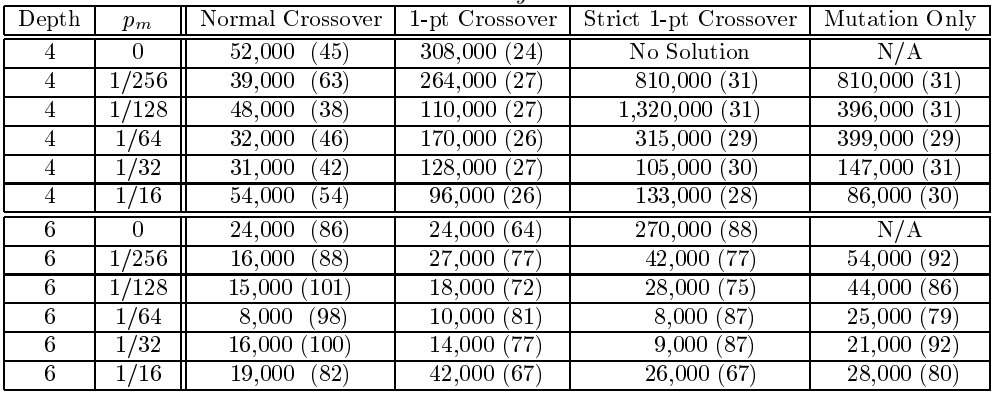
\includegraphics[scale=0.4]{./slike/even3par.png}
	\caption{Rezultati rješavanja 3-paritetnog problema}
	\label{even3par}
\end{figure}

 \begin{figure}[H]
	\centering
	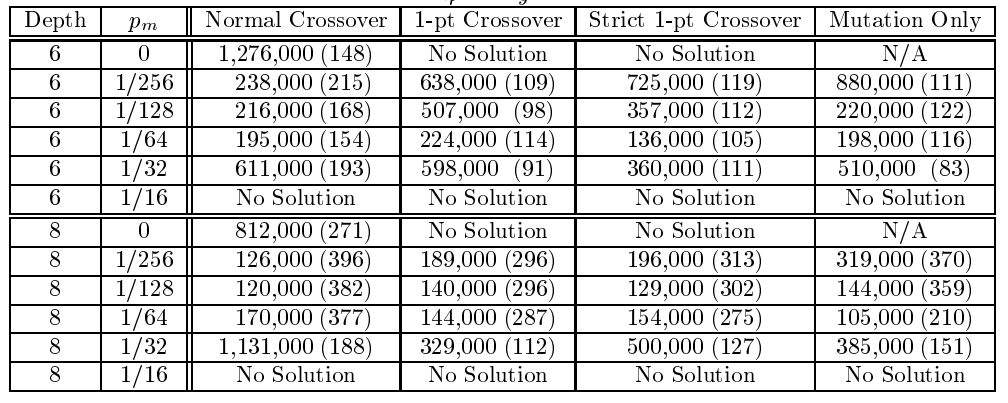
\includegraphics[scale=0.4]{./slike/even4par.png}
	\caption{Rezultati rješavanja 4-paritetnog problema}
	\label{even4par}
\end{figure}


\section{Križanje s očuvanjem konteksta}
Križanje s očuvanjem konteksta \cite{crxContext} također križa dvije jedinke na mjestu točke prekida. Ovaj operator u stablo uvodi koordinate svakog pojedinog čvora. Koordinate označavaju put unutar stabla kojim se dolazi do određenog čvora. Primjer koordinata čvorova stabla dan je na slici \ref{crxContextCoordinates}. Ovakve koordinate jednostavno i jednoznačno opisuju poziciju određenog čvora unutar stabla. Primjerice, čvor s koordinatama (1,1,2) nalazi se u drugoj grani podstabla koje se nalazi u prvoj grani prvog podstabla.

\begin{figure}[H]
 	\centering
\begin{tikzpicture}
	[sibling distance=45mm, level distance=25mm,
	every node/.style={fill=blue!20,circle,draw,drop shadow, minimum height=1.5cm}]
	\node   {-}
    		child {node  {1}
    			child {node {1,1}
    				child {node{1,1,1}}
    				child {node{1,1,2}}
    			}
    		}
    		child {node {2}
        		child {node  {2,1}}
        		child {node {2,2}}
      		};
	};

\end{tikzpicture}


	\caption{Koordinate čvorova stabla}
	\label{crxContextCoordinates}
\end{figure}

\subsection{Križanje s jakim očuvanjem konteksta}
Križanje s jakim očuvanjem konteksta (\textit{eng. strong context preserved crossover - SCPC}) dopušta križanje samo onih podstabala koja imaju potpuno jednake koordinate korijena. Ovakav operator postavlja vrlo stroga ograničenja na proces križanja. U \cite{crxContext} pokazano je kako koristeći ovakav operator, postoji velika vjerojatnost da podstablo generirano na određenoj razini na određenom mjestu stabla nikada ne uspije prijeći u potomke. Ovo bi kroz generacije prouzročilo smanjivanje genetske raznolikosti, što je u potpunoj suprotnosti ulozi operatora križanja. Kako bi se ublažio ovakav utjecaj operatora križanja s jakim očuvanjem konteksta, on se nikada ne koristi ekskluzivno, već u kombinaciji s nekim drugim operatorima križanja.

\subsection{Križanje sa slabim očuvanjem konteksta}
Kako bi se ublažila rigoroznost križanja s jakim očuvanjem konteksta, D'haeseleer \cite{crxContext} je također predložio blažu inačicu ovog križanja - križanje sa slabim očuvanjem konteksta (\textit{eng. weak context preserved crossover - WCPC}). Ova inačica kontekstnog križanja predstavlja pojednostavljenje križanja s jakim očuvanjem konteksta. Korijen podstabla prvog roditelja koje će sudjelovati u križanju odabire se između skupa čvorova za koje postoji odgovarajući čvor u drugom roditelju (jednako kao i kod križanja s jakim očuvanjem konteksta). Podstablo u drugom roditelju koje će sudjelovati u križanju odabire se tako da mu vršni čvor odgovara vršnom čvoru odabranog podstabla prvog roditelja. Drugim riječima, ako su $T1$ i $T2$ važeći odabiri podstabala za križanje s jakim očuvanjem konteksta, tada su $T1$ i $T2' \subseteq T2$ važeći odabiri podstabala za križanje sa slabim očuvanjem konteksta.

\subsection{Dosadašnji rezultati}
U \cite{crxContext} obavljena su četiri različita eksperimenta koja pokazuju učinkovitost ovih operatora križanja. U nastavku su opisani ti eksperimenti.

\subsubsection{Robot sa sposobnosti izmicanja preprekama}
Cilj ovog problema je evoluirati robota koji pi prešao što veću površinu zadanog prostora, zaobilazeći pritom prepreke koje mu se nađu na putu. Pri tome, broj pokreta robota je ograničen na neki fiksni broj $n$. 

Rezultati ovog eksperimenta pokazali su kako ovo križanje nije dobro za evoluciju rješenja danog problema. Budući da evoluirani robot samo jednom izvršava svoj program predstavljen stablom, to stablo bi trebalo biti veliko i opisivati svaki korak robota. Budući da ova križanja, a pogotovo križanje s jakim očuvanjem konteksta ne potiče prijenos krajnjih podstabala rješenja, dobiven rezultat bio je i za očekivati. Na slici \ref{robot} dana je usporedba učinkovitosti uobičajenog (jednostavnog) operatora križanja, kombinacije jednostavnog i križanja s jakim očuvanjem konteksta (u omjeru 1:1) i križanja s jakim očuvanjem konteksta. Vidljivo je kako je jednostavno križanje superiorno nad kontekstnim križanjima za rješavanje ovog problema.

\begin{figure}[H]
	\centering
	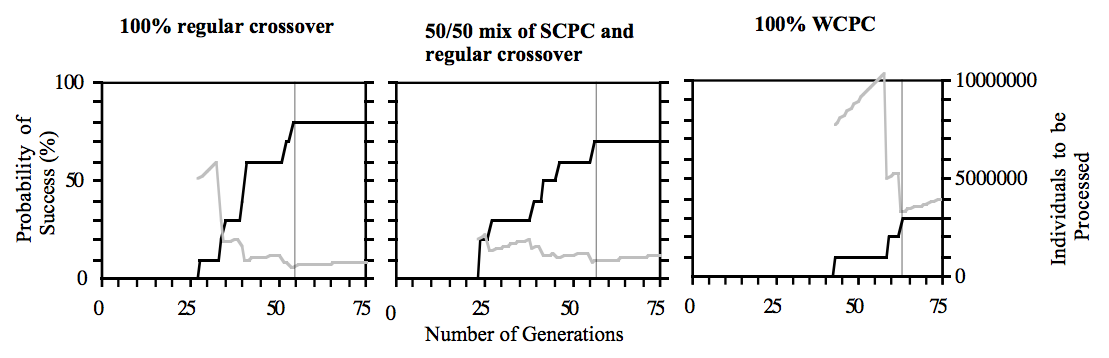
\includegraphics[scale=0.4]{./slike/robot.png}
	\caption{Učinkovitost različitih operatora križanja za problem robota sa sposobnošću izmicanja prepreka. lijevo: jednostavno križanje, sredina: kombinacija jednostavnog i križanja sa slabim očuvanjem konteksta, desno:  križanje s jakim očuvanjem konteksta}
	\label{robot}
\end{figure}


\subsubsection{Iterirana inačica robota sa sposobnosti izmicanja preprekama}
Za razliku od prethodno opisanog problema, gdje se program predstavljen stablom izvršava samo jedan put, u ovom problemu unutar dopuštenog broja koraka dopušteno je izvoditi program po nekoliko puta. Ovakvo ponašanje u stvari je i prirodnije od jednostrukog izvršavanja stabla, i očekivano je da će u ovom slučaju kontekstni operatori djelovati efikasnije nego kod rješavanja prethodnog problema. Na slici \ref{robotIt} prikazana je usporedba učinkovitosti operatora križanja za ovaj problem. Vidljivo je kako je kombinacija jednostavnog i križanja s jakim očuvanjem konteksta (u omjeru 1:3) djelovala najbolje pri rješavanju ovog problema.

\begin{figure}[H]
	\centering
	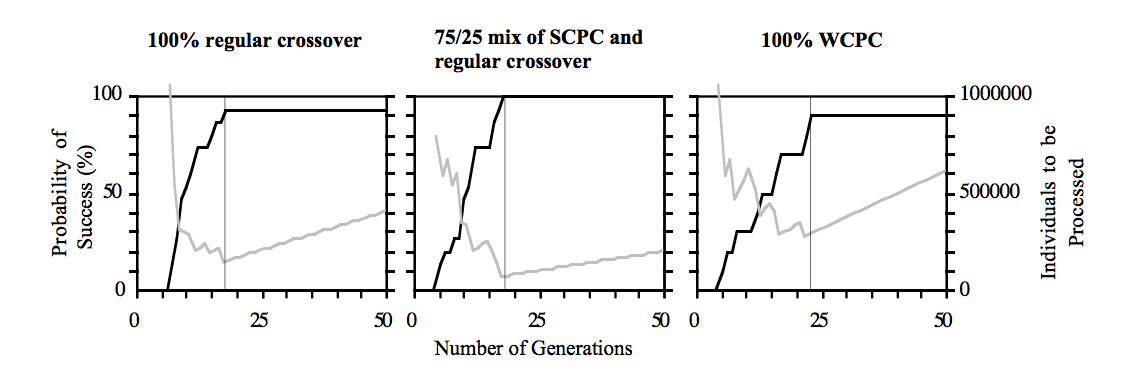
\includegraphics[scale=0.4]{./slike/robotIt.png}
	\caption{Učinkovitost različitih operatora križanja za iterativni problem robota sa sposobnošću izmicanja prepreka. lijevo: jednostavno križanje, sredina: kombinacija jednostavnog i križanja sa slabim očuvanjem konteksta, desno:  križanje s jakim očuvanjem konteksta}
	\label{robotIt}
\end{figure}



\subsubsection{11 - multipleksor}
Cilj boolean 11 - multipleksor problema je pronaći logičku funkciju koja za 3 predana adresna bita daje podatak veličine 8 bita. U ovom problemu, kombinacija jednostavnog i križanja s jakim očuvanjem konteksta (u omjeru 1:1) pokazala se daleko boljim odabirom za operator križanja nego jednostavno križanje. Križanje sa slabim očuvanjem konteksta se i u ovom eksperimentu pokazalo prilično inferiorno ostalim dvama operatorima. Na slici \ref{mux} prikazana je usporedba učinkovitosti različitih operatora križanja na ovaj problem.

\begin{figure}[H]
	\centering
	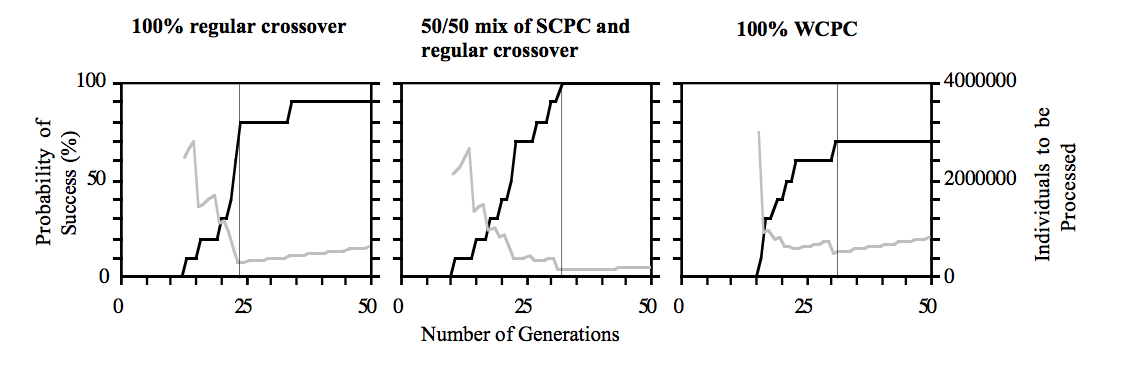
\includegraphics[scale=0.4]{./slike/mux.png}
	\caption{Učinkovitost različitih operatora križanja za problem boolean 11 - multipleksora. lijevo: jednostavno križanje, sredina: kombinacija jednostavnog i križanja sa slabim očuvanjem konteksta, desno:  križanje s jakim očuvanjem konteksta}
	\label{mux}
\end{figure}



\subsubsection{Centralno sakupljalište hrane}
Efikasno rješenje ovog problema je evoluirani program koji, kada je pokrenut nad svakim umjetnim mravom kolonije, prouzrokuje transport sve hrane s danog područja na jedno, centralno mjesto. Dobro rješenje ovog problema mora uključivati i interakciju i kooperaciju između mrava. Radi toga, evoluirani program najčešće su kratki, sadržavajući samo nekoliko koraka u svakoj iteraciji izvođenja. Ovo upućuje na činjenicu da bi kontekstno križanje moglo biti vrlo korisno za evoluciju takvog, efikasnog rješenja. Na slici \ref{ants}, jednako kao i za prethodne eksperimente, prikazana je usporedba učinkovitosti različitih operatora križanja na ovaj problem.

\begin{figure}[H]
	\centering
	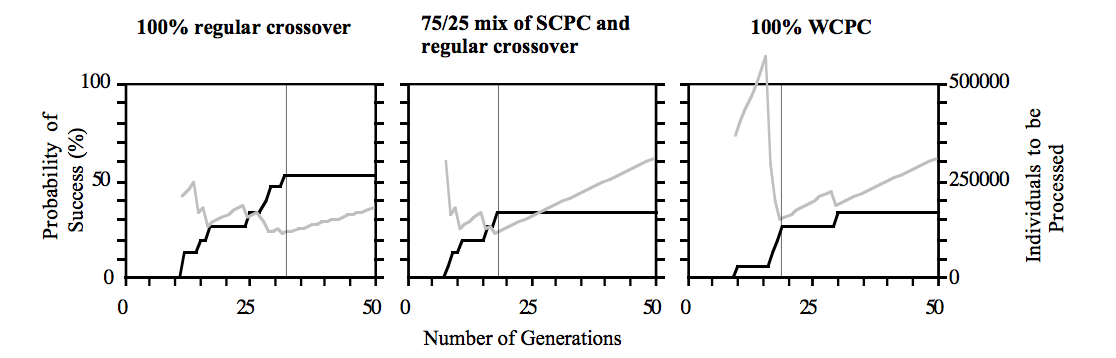
\includegraphics[scale=0.4]{./slike/ants.png}
	\caption{Učinkovitost različitih operatora križanja za problem centralnog sakupljališta hrane. lijevo: jednostavno križanje, sredina: kombinacija jednostavnog i križanja sa slabim očuvanjem konteksta, desno:  križanje s jakim očuvanjem konteksta}
	\label{ants}
\end{figure}



Ova istraživanja pokazala su kako križanje s očuvanjem konteksta nije učinkovito kada je upotrebljeno samo, već je efikasnije u kombinaciji s nekim drugim operatorom. Kombinacija jednostavnog križanja i križanja s jakim očuvanjem konteksta pokazala se kao vrlo učinkovit operator za iterirane programe koji predstavljaju neovisnu jedinku i za pronalazak logičkih funkcija.



\section{Križanje pravedno s obzirom na veličinu}
Česta pojava u genetskom programiranju je prekomjeran rast jedinki kako teku generacije (\textit{eng. bloat}). Postoji više načina rješavanja ili sprječavanja ovog problema. Jedan od načina kako riješiti ovaj problem nad već generiranim jedinkama je podrezivanje (\textit{eng. pruning}), odnosno odstranjivanje onih dijelova stabla koji su izvan dopuštene dubine. Drugi način je da se rezultat operatora križanja odbacuje sve dok je stablo producirano takvim križanjem veće dubine nego što je dopušteno. Moguće je i kažnjavati predugačka rješenja umanjivanjem njihove dobrote. Ovaj operator taj problem rješava u samom postupku križanja. Naime, kontrolirajući veličinu podstabala koja ulaze u križanje, direktno kontrolira veličinu novogeneriranog potomka.

Nakon što je algoritam dosegnuo stagnaciju u napredovanju, uobičajeni operatori križanja pokušat će proširiti prostor pretrage. No, radi pojave prekomjernog rasta, ova potraga više će se protezati u prostoru duljine samog rješenja nego u prostoru različitih rješenja. Kod ovakvog pristupa, postoji veća vjerojatnost za preživljavanjem dijelova rješenja koji nisu štetni, ali nisu ni korisni - podržavajući tako daljnji rast jedinki. Kod križanja pravednog s obzirom na veličinu, to nije slučaj - nakon dosegnutog platoa, ono će istraživati različita rješenja, čisto iz razloga što je jedinka dobivena ovakvim križanjem otprilike jednake veličine kao i svoji roditelji.

U \cite{crxSizeFair} predstavljeno je križanje pravedno s obzirom na veličinu. Odabir točke prekida u prvom roditelju koji sudjeluje u križanju obavlja se nasumično. Pri tome, pristranost odabiru nezavršnog čvora stabla nad odabirom lista stabla iznosi 0.9. Ono po čemu se ovo križanje razlikuje od jednostavnog križanja je odabir točke prekida u drugom roditelju. Kako bi se pronašla druga točka prekida, izračunava se veličina stabla koje će biti obrisano u kopiji prvog roditelja. Nakon toga, u drugom stablu pronalaze se podstabla veličine ne veće od $1+2 \cdot |veličina\_obrisanog\_podstabla|$. Ovime se osigurava da novostvorena jedinka neće biti veća od $veličina\_prvog\_roditelja + |veličina\_obrisanog\_podstabla| + 1$.



\subsection{Dosadašnji rezultati}
U \cite{crxSizeFair}  provedeno je istraživanje nad četiri različita problema; po dva za simboličku regresiju (polinomi petog i šestog stupnja) i po dva za logičke funkcije (6 i 11 - multipleksor). Pokazano je kako je ovaj operator križanja kroz generacije proizvodio značajno, pa čak i do deset puta manje jedinke nego jednostavni operator križanja. Uočeno je da je u slučaju kada se početna populacija sastoji od jedinki koje su puno manje nego što je potrebno, jednostavno križanje i dalje superiornije pri pronalasku rješenja. Ovo se može pokazati kao značajan nedostatak ukoliko se na početku algoritma ne poznaje okvirna veličina dobrog rješenja. Dokazano je da ovaj operator značajno smanjuje prekomjeran rast jedinki. Za usporedbu, prosječan rast jedinki tijekom generacija za jednostavno križanje je linearno, dok je prosječan rast jedinki za ovo križanje subkvadratno.

\section{Uniformno križanje}
Uniformno križanje predstavljeno je u \cite{crxUniform}. Inspirirano je uniformnim križanjem nestablastih struktura u genetskom algoritmu. U genetskom algoritmu, ovo križanje (budući da su sve jedinke jednakih dužina) prolazi kroz oba roditelja te na svakoj poziciji nasumično odabire gen iz prvog ili drugog roditelja te ga ugrađuje u dijete. Kada bi u genetskom programiranju sve jedinke bile potpuno jednakog oblika, ovo križanje funkcioniralo bi potpuno jednako. No, budući da je to vrlo rijedak slučaj, potrebno je, kao i u križanju s jednom točkom prekida, pronaći zajedničko područje dva roditelja. Nakon što je to područje pronađeno, s lakoćom se smiju izmjenjivati čvorovi roditeljskih stabala - no pritom je potrebno paziti na broj djece koji taj čvor posjeduje. Na slici \ref{crxUni} prikazan je primjer jednog mogućeg rezultata uniformnog križanja.

\begin{figure}[H]
 	\centering


\begin{tikzpicture}
	[sibling distance=25mm, level distance=15mm,
	every node/.style={fill=blue!20,circle,draw,drop shadow, minimum height=1cm}]

\begin{scope}[xshift=0cm]

	\node  [fill=yellow!20]  {\textbf{+}}
    		child {node [fill=yellow!20]  {$cos$}
    			child {node  [fill=yellow!20] {-}
    				child {node{x}}
    				child {node{y}}
    			}
    		}
    		child {node [fill=yellow!20]  {\textbf{$\cdot$}}
        		child {node [fill=yellow!20]  {2}}
        		child {node [fill=yellow!20]  {y}}
      		};
	};
\end{scope}

\begin{scope}[xshift=7cm]
	\node  [fill=yellow!20]  {\textbf{+}}
    		child {node  [fill=yellow!20] {$sin$}
        		child {node  [fill=yellow!20] {y}}
      		}
    		child {node [fill=yellow!20] {\textbf{$/$}}
			child {node [fill=yellow!20]  {x}}
			child {node [fill=yellow!20]  {y}}	
		};
	};
\end{scope}

\end{tikzpicture}


	\caption{Zajedničko područje dva roditelja}
	\label{crxOnePointCommon}
\end{figure}

\begin{figure}[H]
 	\centering


\begin{tikzpicture}
	[sibling distance=25mm, level distance=15mm,
	every node/.style={fill=blue!20,circle,draw,drop shadow, minimum height=1cm}]

\begin{scope}[xshift=0cm]

	\node {\textbf{+}}
    		child {node [fill=red!20]  {$sin$}
    				child {node{-}
    					child {node {x}}
    					child {node {y}}
    			}
    		}
    		child {node  [fill=red!20] {\textbf{$/$}}
        		child {node [fill=red!20]  {x}}
        		child {node {y}}
      		};
	};
\end{scope}

\begin{scope}[xshift=7cm]
	\node   {\textbf{+}}
    		child {node  [fill=red!20] {$sin$}
        		child {node  [fill=red!20] {y}}
      		}
    		child {node  [fill=red!20]  {\textbf{$\cdot$}}
			child {node  {x}}
			child {node  {y}}	
		};
	};
\end{scope}

\end{tikzpicture}


	\caption{Mogući rezultati križanja roditelja sa slike \ref{crxOnePointCommon}}
	\label{crxUni}
\end{figure}

Velika prednost ovog križanja je velika stopa razmjene genetskog materijala. Budući da se čvorovi koji će završiti u djetetu biraju uniformno, s omjerima vjerojatnosti 1:1, velika je vjerojatnost da će dijete sadržavati 50\% genetskog materijala prvog roditelja i 50\% genetskog materijala drugog roditelja. Ovo je vrlo pogodno za brzo napredovanje algoritma.

\subsection{Dosadašnji rezultati}
Autor ovog križanja proveo je eksperimente nad paritetnim problemom 4 varijable. Cilj ovog problema je pronaći logičku funkciju koja je istinita za parni broj istinitih varijabli. Tablica istinitosti za ovaj problem prikazana je na tablici ispod (\ref{truthTable}).

\begin{table}[H]
\centering

\begin{tabular} {a b c d | p}
A & B & C & D & P \\
\hline
0 & 0 & 0 & 0 & 1 \\
0 & 0 & 0 & 1 & 0 \\
0 & 0 & 1 & 0 & 0 \\
0 & 0 & 1 & 1 & 1 \\
0 & 1 & 0 & 0 & 0 \\
0 & 1 & 0 & 1 & 1 \\
0 & 1 & 1 & 0 & 1 \\
0 & 1 & 1 & 1 & 0 \\
1 & 0 & 0 & 0 & 0 \\
1 & 0 & 0 & 1 & 1 \\
1 & 0 & 1 & 0 & 1 \\
1 & 0 & 1 & 1 & 0 \\
1 & 1 & 0 & 0 & 1 \\
1 & 1 & 0 & 1 & 0 \\
1 & 1 & 1 & 0 & 0 \\
1 & 1 & 1 & 1 & 1 \\
\hline
\end{tabular}

	\caption{Tablica istinitosti za paritetni problem 4 varijable}
	\label{truthTable}
\end{table}

Eksperimentima je dokazano kako za razliku od jednostavnog križanja i križanja s jednom točkom prekida, u kojima je prosječna stopa razmjene genetskog materijala oko 5\%, ovo križanje uistinu ima konstantnu stopu razmjene genetskog materijala od oko 50\%.

Pokazano je kako jednostavno križanje pretragu prostora rješenja odvija lokalno, nasljeđujući većinu genetskog materijala od jednog roditelja. Jednostavno križanje nije idealno za brzo pretraživanje prostora - bolje je za fino ugođavanje prilično dobrog rješenja. Osim toga, jednostavno križanje vrlo lako zapne u nekom od lokalnih optimuma. 

Križanje s jednom točkom prekida bolje se nosi s veličinom prostora pretrage, no nakon nekog vremena počinje sagledavati sve manji dio prostora - lokalizirajući tako pretragu s povećanjem vjerojatnosti zapinjanja u lokalnom optimumu.

Uniformno križanje prelazi preko ovih problema. Za razliku od jednostavnog križanja, ono nije pristrano na križanje listova ili podstabala. Ovime omogućuje slobodniju i raznolikiju izmjenu genetskog materijala između roditelja, ubrzavajući tako konvergenciju rješenja u globalni optimum. Također, pokazano je kako nakon nekog vremena, sve jednike populacije budu otprilike jednake veličine, što kod upotrebe jednostavnog križanja i križanja s jednom točkom prekida nije slučaj. Osim navedenih svojstava, nije uočena prevelika razlika u samoj uspješnosti križanja da pronađe dobro rješenje problema - rad se pretežito fokusirao na razliku u količini izmijenjenog genetskog materijala.



\section{Homologno križanje}
Homologno križanje \cite{crxSizeFair} temelji se na prirodnom svojstvu križanja, homologiji. Homologija u prirodi osigurava da se križanje uvijek događa između organizama koji imaju uglavnom identične sekvence gena unutar kromosoma. Ovime se podupire nedestruktivno križanje - kombiniraju se geni koji rade točno određenu ulogu, gdje je uloga uvjetovana pozicijom samog gena.

Homologno križanje, u smislu križanja u genetskom programiranju, koristi pozicijsku homologiju. Pozicijska homologija potiče izmjenu genetskog materijala samo ako se ono događa na istoj, ili dovoljno bliskoj poziciji unutar dva genoma.

Uobičajeni operatori križanja, prilikom odabira podstabala ili čvorova koji sudjeluju u križanju uglavnom ne uzimaju u obzir njihovu poziciju. Ne uzimajući to u obzir, nerijetko dolazi do naglog rasta jedinki svakom novom generacijom (\textit{eng. bloat}). Budući da ovi operatori najčešće ne uzimaju u obzir prekomjeran rast jedinki koje proizvode, potrebno je modificirati sam algoritam tako da se prevelike jedinke kažnjavaju manjom dobrotom. Time, iako možda novonastala jedinka izvrsno rješava zadan problem, može se dogoditi da bude odbačena zbog svoje veličine. Iz razloga što se ne uzimaju u obzir pozicije niti veličine podstabala koja sudjeluju u križanju, mala je šansa da će novonastala jedinka biti u okviru željene veličine, povećavajući šansu da će u budućnosti zbog te veličine i izumrijeti. Drugi razlog zbog kojega prekomjeran rast jedinke nije dobar, a usko je povezan s prethodnim, je taj da, u prevelikoj jedinci vjerojatno postoji puno nepotrebnog ponašanja - ponašanje koje nije potrebno, a kroz generacije je preživjelo samo zato što ne donosi nikakvu štetu.

Drugi problem koji se javlja kod uobičajenih operatora križanja je taj da ti operatori potpuno nasumično prenose dijelove programa u novu jedinku. Budući da je taj fragment jedinke preživio proces selekcije, za pretpostaviti je da postoji velika šansa da on predstavlja relevantan dio za put do konačnog rješenja. Također, velika je šansa da korisnost istog fragmenta uvelike ovisi i o kontekstu u kojem se on izvršava. Stavljajući takav fragment na nasumično mjesto u novu jedinku donosi šansu da će taj kontekst biti uništen.

Kako bi se ovi problemi riješili prilikom samog križanja, a time se i povećale šanse za kvalitetu i nastavak života potomaka, homologni operator križanja prilikom samog križanja uzima u obzir i veličinu i poziciju podstabala roditelja koja će se iskrižati. Ovime se u samoj srži operatora sprječava prekomjeran rast potomaka i s većom vjerojatnošću nego inače, podržava prijenos konteksta pojedinih fragmenata rješenja u ono novonastalo.

Ovo križanje u stvari je inačica križanja pravednog s obzirom na veličinu. Odabir potencijalnih podstabala drugog roditelja potpuno je jednak u ovom križanju kao i kod križanja pravednog s obzirom na veličinu. Razlika u tome je ta da se, između svih potencijalnih podstabala drugog roditelja koji bi mogli sudjelovati u križanju, odabire ono podstablo koje je najbliže točki prekida prvog roditelja. Na slici \ref{crxHomo} prikazan je jedan takav primjer križanja - od dva potencijalna podstabala drugog roditelja, za križanje je odabrano ono koje je bliže točki prekida u prvom roditelju.

\begin{figure}[H]
	\centering
	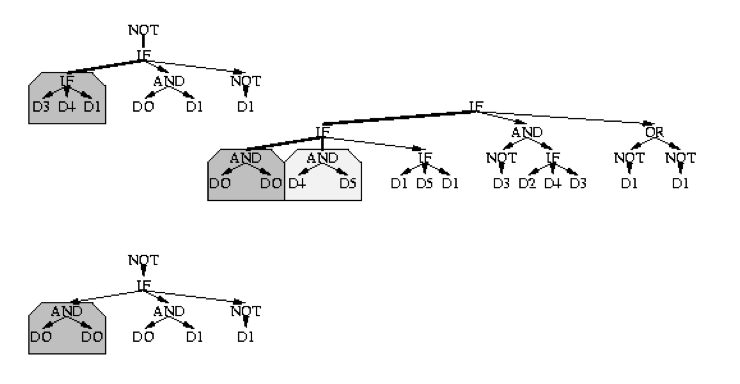
\includegraphics[scale=0.6]{./slike/crxHomo.png}
	\caption{Primjer homolognog križanja (preuzeto iz  \cite{crxSizeFair})}
	\label{crxHomo}
\end{figure}

\subsection{Dosadašnji rezultati}
U \cite{crxSizeFair}  provedeno je istraživanje nad četiri različita problema; po dva za simboličku regresiju (polinomi petog i šestog stupnja) i po dva za logičke funkcije (6 i 11 - multipleksor). Pokazano je kako homologno križanje po sposobnosti pronalaska rješenja danih problema nije značajno bolje od križanja pravednog s obzirom na veličinu. No, kao i kod križanja pravednog s obzirom na veličinu, pokazano je kako je ovo križanje vrlo učinkovito prilikom sprječavanja pojave prekomjernog rasta jedinki.

Razlog sličnosti u rezultatima s križanjem pravednim s obzirom na veličini može biti prouzrokovano različitim razlozima. Jedan od razloga je mogućnost da kod ovog operatora u nekim slučajevima nije postojao izbor podstabla koji bi bio u skladu s homologijom, te bi operator bio primoran odabrati podstablo koje ne odgovara u potpunosti načelu odabira. Postojanje ovog slučaja pokazano je u spomenutom radu.



\section{Determinističko križanje}
Determinističko križanje (\textit{eng. deterministic functional crossover}), opisano u \cite{crxDeter}, ostvaruje križanje dvije jedinke na osnovi funkcijske sličnosti. Ovaj operator primjenjiv je samo na probleme simboličke regresije.

Kako bi se funkcijska sličnost dva gena, odnosno čvorova stabla koji izgrađuju jedinku, mogla odrediti, za svaki gen zapisuje se minimalna i maksimalna vrijednost koju može poprimiti za podatke iz skupa za učenje. Funkcijska sličnost (u radu nazvana funkcijskom udaljenošću) između dva gena i i j, računa se kao:

\begin{equation} 
\label{udaljenost}
 \large{ d_{i,j} = \frac{1}{2} (|max_i - max_j| + |min_i - min_j|) }
\end{equation}
\\
U radu je opisan glavni nedostatak ovog križanja - postoji velika vjerojatnost da križanje koje se dogodi pod utjecajem ovog operatora bude neutralno, odnosno, da se novonastala jedinka uopće ne razlikuje od jednog od roditelja. Ovaj slučaj dogodi se kada se u prvom roditelju izabere podstablo koje je strukturno jednako odabranom podstablu drugog roditelja (može biti interpretirano na jednak način nakon što se izraz predstavljen podstablom simplificira). Križanjem takvih podstabala, originalno ponašanje se uopće ne mijenja te je rezultantna jedinka potpuno jednaka svome roditelju. Pojava neutralnog križanja to je češća što jedinke sve više i više rastu (čime se povećava vjerojatnost odabira strukturno jednakog podstabla). Kako bi se riješio ovaj problem, u istom radu predloženo je probabilističko križanje, koje je opisano u idućem poglavlju.

\subsection{Dosadašnji rezultati}
Na slici \ref{deto} prikazani su grafovi usporedbe učinkovitost determinističkog križanja u usporedbi s jednostavnim i probabilističkim križanjem i slučaja kada nije upotrijebljen niti jedan operator križanja. Pri tome, grafovi na lijevoj strani pokazuju performanse dobivenih rješenja na skupu za učenje, a oni na desnoj strani, performanse na skupu za testiranje. Eksperimenti su bili provedeni na primjerima simboličke regresije. Na desnoj strani slike, vidljivo je kako ne postoji prevelika razlika između učinkovitosti danih operatora. 


\begin{figure}[H]
	\centering
	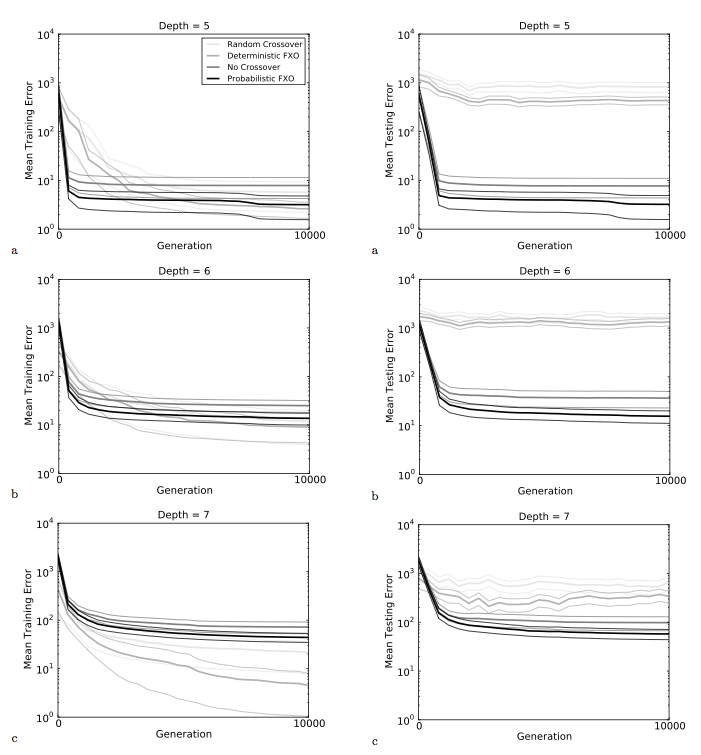
\includegraphics[scale=0.65]{./slike/deto.png}
	\caption{Usporedba učinkovitosti determinističkog, jednostavnog i probabilističkog križanja i slučaja kada nije upotrijebljen niti jedan operator križanja (preuzeto iz \cite{crxDeter})}
	\label{deto}
\end{figure}

Također, vidljivo je kako je ovo križanje dalo superiorno rješenje na skupu za učenje naspram ostalima za slučaj kada je dubina stabla jednaka 7. U suprotnosti, odnosno, posljedično tome, na skupu za testiranje isti slučaj dao je značajno slabije rezultate što upućuje na prenaučavanje jedinki.

Također, pokazano je da ovo križanje ne podržava prekomjeran rast jedinki tijekom generacije. Dapače, dana rješenja često su ispala nešto manja od onog ciljanog.




\section{Probabilističko križanje}

Kako bi se riješio problem neutralnog križanja koji se pojavio kod determinističkog križanja, u \cite{crxDeter} je predloženo probabilističko križanje (\textit{eng. probabilistic functional crossover}). Jednako kao i kod determinističkog križanja, za svaki čvor u stablu zapisuje se minimalna i maksimalna vrijednost čvora za podatke iz skupa za učenje (izraz \ref{udaljenost}).

Prilikom križanja, nakon što se u prvom stablu nasumično odabere točka križanja izračunava se funkcionalna udaljenost između njega i svakog čvora unutar drugog roditelja (jednako kao i kod determinističkog križanja). Nakon što su dobivene sve moguće udaljenosti, one se normaliziraju prema \ref{norm}:

\begin{equation} 
\label{norm}
 \large{ d '_{i,j} = \frac{d_{i,j}}{\sum_{k=1}^{s} d_{i,k}} }
\end{equation}
 
Normalizacija je pogodna iz razloga što se s najvećom vjerojatnošću želi odabrati funkcionalno najbliži čvor. Ovako dobivene normalizirane udaljenosti potom se invertiraju i ponovno normaliziraju u odnosu na te invertirane vrijednosti prema \ref{prob}:
 
 \begin{equation} 
\label{prob}
 \large{ p_{i,j} = \frac{1 - d '_{i,j}}{\sum_{k=1}^{s} (1 - d '_{i,k})} }
\end{equation}

Time dobivamo to veću vjerojatnost što je udaljenost između dva čvora manja. Nakon ovih operacija, nasumično, ali s izračunatim vjerojatnostima, odabire se podstablo unutar drugog roditelja koje će se iskoristiti za križanje. Pokazano je kako ovakvo križanje pridonosi većem postotku korisnog križanja, a time i bržoj konvergenciji nego uobičajeni operatori, iako je priznato kako je ovakav izračun udaljenosti prilično gruba aproksimacija funkcionalne udaljenosti.

\subsection{Dosadašnji rezultati}
Jednako kao i za determinističko križanje, provedeni eksperimenti za ovo križanje uključuju usporedbu probabilističkog, determinističkog i jednostavnog križanja i slučaja kada nije upotrijebljen niti jedan operator križanja. Rezultati su prikazani su na slici \ref{deto}. Vidljivo je kako probabilističko križanje konstantno bolje djeluje od jednostavnog križanja i slučaja kada se ne koristi niti jedan operator križanja.

Osim toga, dokazano je kako je korisnost križanja \footnote{križanje se smatra korisnim ukoliko producira jedinku koja ima dobrotu bolju od oba roditelja}, kada se koristi probabilistički operator križanja, puno veća nego u ostalim slučajevima. Pokazano je kako se ovim križanjem dobivaju jedinke koje su značajno veće od točnog rješenja. Naravno, pitanje je kako interpretirati ovu pojavu, budući da se izraz koji predstavlja jedinka gotovo uvijek može pojednostavniti čime bi stablo bilo puno manje.

Uočena je korelacija između veličine roditelja i događanja korisnog križanja. No, to je i za očekivati iz razloga što je omjer broja listova na prema unutarnjim čvorovima to veći što je samo stablo veće. Radi toga, vjerojatnost odabira lista za ulazak u križanje se povećava, čime se i smanjuje mogućnost za destruktivnim križanjem. 

\section{Semantičko križanje}
Suprotstavljeno tradicionalnim operatorima križanja u genetskom programiranju koji ignoriraju semantiku samog programa, u \cite{crxSem} opisano je semantičko križanje. 
Ovo križanje razlikuje nekoliko inačica, od kojih je svaka primjenjiva na određenu vrstu problema. Semantičko križanje različito je definirano za situacije kada stablo jedinke predstavlja logičku ili realnu funkciju, ili ako je jedinka program.

Ukoliko jedinka predstavlja logičku funkciju, semantičko križanje definirano je kao:
 \begin{equation} 
\label{log}
 \large{ (T1 \land T2) \vee   (\overline{TR} \land T2) },
\end{equation}
gdje T1 i T2 predstavljaju roditelje koji sudjeluju u križanju, a TR predstavlja nasumično generirano stablo. Na slici \ref{semBool} prikazana je shema semantičkog križanja za logičke funckije.

 \begin{figure}[H]
	\centering
	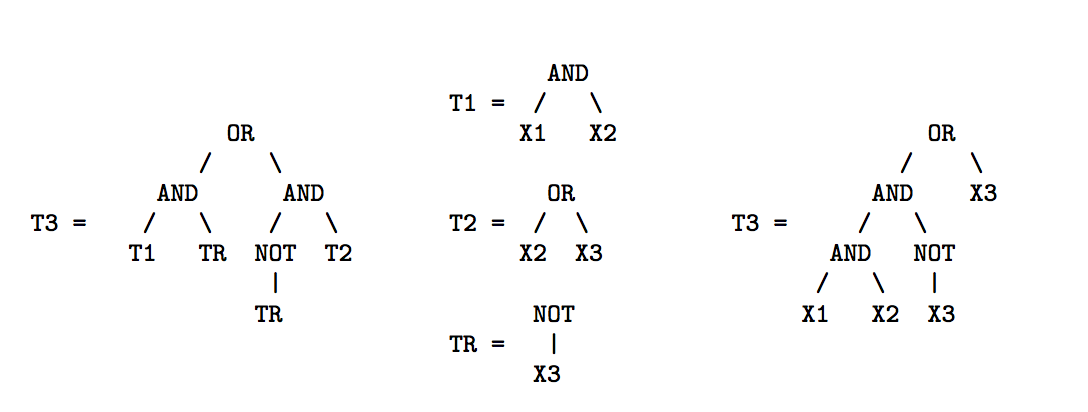
\includegraphics[scale=0.4]{./slike/semBool1.png}
	\caption{Lijevo: shema semantičkog križanja za logičke funkcije; sredina: roditelji i nasumično generirana jedinka; desno: rezultat križanja roditelja prikazanih u sredini }
	\label{semBool}
\end{figure}
  
   
     Analogno ovome, za realne funkcije, odnosno, simboličku regresiju, semantičko križanje predstavljeno je sljedećim izrazom:
 \begin{equation} 
\label{log}
 \large{ (T1 \cdot T2) +   ((1-TR) \cdot T2) }.
\end{equation}
Za slučaj kada jedinka predstavlja program, semantičko križanje definira se kao:
 \begin{equation} 
\label{log}
 \large{ \textbf{IF}(CONDR) \textbf{THEN} (T1) \textbf{ELSE} (T2)},
\end{equation}
gdje je CONDR nasumično generiran program čiji je izlaz interpretiran kao logička vrijednost.

Iz ovoga je jasno vidljiv najveći nedostatak ovog operatora - prekomjeran rast novonastalih jedinki. Naime, prilikom svakog križanja stablo će se sigurno uvećati po dubini za barem jednu razinu. Ovo može postati znatan problem iz razloga što je rast vrlo brz, te se često nakon nekog vremena dogodi to da za novodobiveno stablo ne postoji prostor za pohranu. Radi ovoga, nakon svakog križanja, potrebno je pojednostavniti novonastalu jedinku. Ovo pojednostavljenje naravno mora osigurati da je funkcionalnost jedinke nakon pojednostavljenja ostala nepromijenjena.

Glavna prednost ovog semantičkog operatora je činjenica da je, za razliku od nekih drugih predloženih semantičkih operatora, primjenjiv na širok skup problema.

\subsection{Dosadašnji rezultati}

Eksperimenti u \cite{crxSem} provedeni su nad sve tri vrste problema za koje je ovaj operator definiran; logičke funkcije, simboličku regresiju i programe. Ovo istraživanje je usporedilo genetsko programiranje (\texit{GP}) sa semantičkim genetskim programiranjem (\textit{eng. semantic genetic programming - SGP}) i semantičkim stohastičkim planinskim penjačem (\textit{semantic stochastic hill climber - SSHC}). Također, napravljena je usporedba s algoritmom genetskog programiranja koje se vrti jednako dugo kao i SGP i SSHC za pojedini problem (\textit{GPt}). U nastavku su opisani dobiveni rezultati za pojedinu vrstu problema.

\subsubsection{Logičke funkcije}

Učinkovitost logičkog semantičkog operatora križanja provedena je na 5 različita problema, zajedno s nekoliko inačica za svaki problem. Problemi su redom: $n$ -komparator (6, 8 i 10), $n$ -multipleksor (6 i 11), $n$ -paritet (5, 6, 7, 8, 9 i 10), nasumično generirana funkcija $n$ varijabli (5, 6, 7, 8, 9, 10 i 11) i $n$-istinita funkcija \footnote{$n$-istinita funkcija je funkcija $n$ varijabli koja je za svaku kombinaciju varijabli istinita} (5, 6, 7 i 8). Dobrota je računata kao Hammingova udaljenost vrijednosti stvarne funkcije i dobivenog rješenja. Na slici \ref{semBoolTable} prikazana je tablica rezultata. 

Stupac \textit{Hits \%} predstavlja postotak uspješnosti nad skupom za učenje za najbolju jedinku u populaciji, za 30 pokretanja algoritma. Pri tome \textit{avg} predstavlja prosjek, a \textit{sd} standardnu devijaciju. U stupcu \textit{Length} prikazani su logaritmi po bazi 10 veličine dobivenih rješenja. Valja napomenuti da je nakon upotrebe semantičkog križanja primijenjena simplifikacija dobivenog rješenja, iz razloga što bi veličina rješenja eksponencijalno rasla u suprotnom. Vidljivo je kako SSHC i SGP konstantno pronalaze bolja rješenja od GP-a sa semantičkim križanjem, no GP proizvodi manje jedinke (čemu je glavni razlog pojednostavljenje izraza koje se u ostalim algoritmima ne obavlja - što umanjuje relevantnost ovog zaključka).  Vidljivo je kako GPt pokazuje bolje performanse od GP-a, no još uvijek se pokazuje lošijim od SGP-a i SSHC-a.

 \begin{figure}[H]
	\centering
	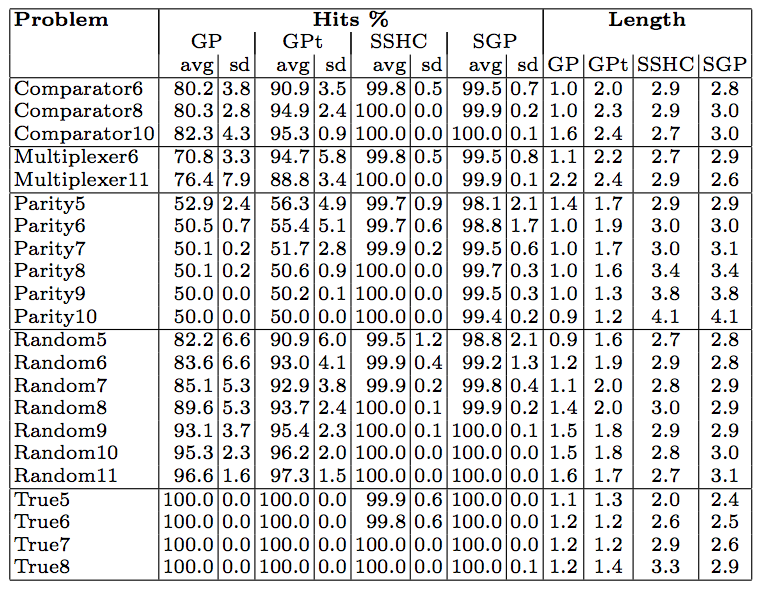
\includegraphics[scale=0.5]{./slike/semBoolTable.png}
	\caption{Usporedba učinkovitosti GP-a i GPt-a sa SGP-om i SSHC-om}
	\label{semBoolTable}
\end{figure}

\subsubsection{Simbolička regresija}

Za ocjenu učinkovitosti ovog operatora na simboličkoj regresiji korišteni su različiti polinomi, od trećeg do desetog stupnja, s koeficijentima realnih vrijednosti iz intervala $[-1, 1]$. Funkcija dobrote računata je kao euklidska udaljenost stvarne funkcije i pronađenog rješenja. Na slici \ref{semSymbTable} prikazane su dobivene statistike provedenih eksperimenata.

 \begin{figure}[H]
	\centering
	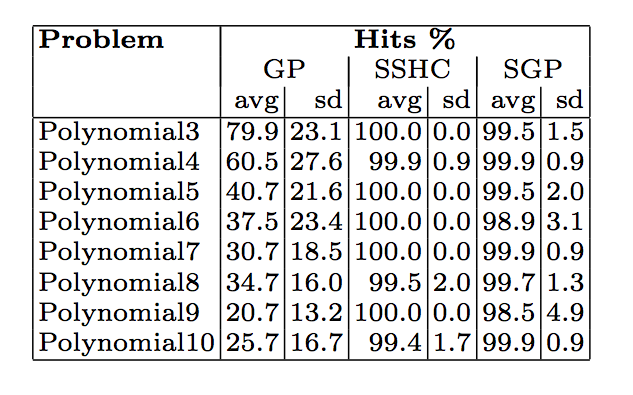
\includegraphics[scale=0.4]{./slike/semSymbTable.png}
	\caption{Usporedba učinkovitosti GP-a i GPt-a sa SGP-om i SSHC-om}
	\label{semSymbTable}
\end{figure}

Vidljivo je kako je GP kao i u prethodnom slučaju, gori od SSHC-a i SGP-a, te da je standardna devijacija dosta veća nego kod ostalih.

\subsubsection{Programi}

Kako bi se pokazala učinkovitost semantičkog križanja nad programskim jedinkama, korišten je problem klasifikacije u jednu klasu na osnovu dvije značajke ($(n_c, n_v) \to n_ {cl}$). Na slici \ref{semProg} prikazani su rezultati eksperimenata. Ovdje je ponovno pokazana inferiornost GP-a naprema SSHC-u i SGP-u.

 \begin{figure}[H]
	\centering
	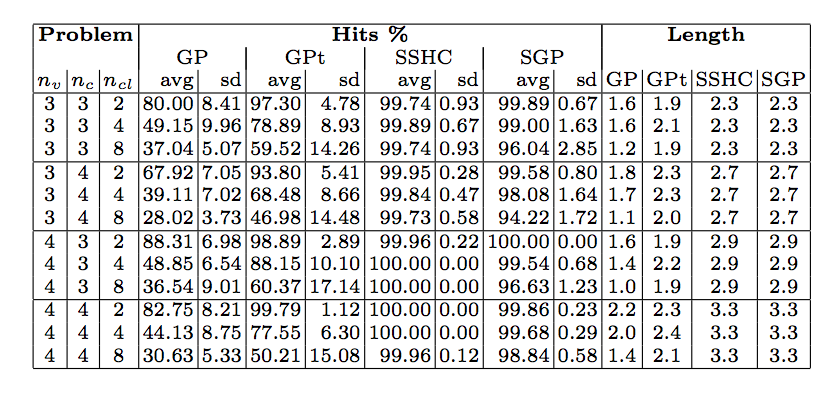
\includegraphics[scale=0.5]{./slike/semProg.png}
	\caption{Usporedba učinkovitosti GP-a i GPt-a sa SGP-om i SSHC-om}
	\label{semProg}
\end{figure}

Unatoč prikazanim rezultatima, autori \cite{crxSem} tvrde da ovaj operator križanja djeluje bolje od uobičajenih operatora u genetskom programiranju. No, za to nisu priložili nikakav dokaz. U sklopu ovog rada implementirano je ovakvo križanje, te će u kasnijim poglavljima biti prikazana usporedba učinkovitosti ovog operatora s onim operatorima koji su opisani u prethodnim poglavljima.